\documentclass[12pt,a4paper,openright,twoside]{book}
\usepackage[italian,english]{babel}
\usepackage[utf8]{inputenc}
\usepackage{disi-thesis}
\usepackage{code-lstlistings}
\usepackage{notes}
\usepackage{shortcuts}
\usepackage{acronym}
\usepackage{float}
\usepackage{pgfplots}

\school{\unibo}
\programme{Corso di Laurea in Ingegneria e Scienze Informatiche}
\title{Kotlin Multiplatform e PulvReAKt: analisi e prototipazione di applicazioni IoT eterogenee}
\author{Coli Alessandro}
\date{\today}
\subject{Programmazione ad Oggetti}
\supervisor{Prof. Viroli Mirko}
\cosupervisor{Dott. Farabegoli Nicolas}
\session{I}
\academicyear{2023-2024}

% Definition of acronyms
\acrodef{IoT}{Internet of Thing}
\acrodef{JVM}{Java Virtual Machine}
\acrodef{JS}{JavaScript}
\acrodef{MQTT}{Message Queuing Telemetry Transport}
\acrodef{QoS}{Quality of Service}
\acrodef{CI/CD}{Continuous Integration and Continuous Deployment}
\acrodef{TCP}{Transmission Control Protocol}

\mainlinespacing{1.241}

\begin{document}
\selectlanguage{italian}

\frontmatter\frontispiece

\begin{dedication}
A te che ci sei sempre stato\\
e sempre sei con me anche se te ne sei andato.\\
A te che tanto mi hai insegnato\\
e sempre mi hai supportato.
\bigbreak
A te che più di chiunque altro avrei voluto qua.
\smallbreak
A mio nonno Gianni.
\end{dedication}

%----------------------------------------------------------------------------------------
\tableofcontents
\listoffigures
%\lstlistoflistings
%----------------------------------------------------------------------------------------

\mainmatter

%----------------------------------------------------------------------------------------
\chapter{Introduzione}
\label{chap:Introduzione}
%----------------------------------------------------------------------------------------
\paragraph{Structure of the Thesis}
\note{At the end, describe the structure of the paper}

\chapter{Contesto}\label{chap:Contesto}

\section{Sviluppo Multiplatform}

Lo sviluppo multiplatform è diventato un approccio sempre più diffuso per la creazione di applicazioni che devono essere eseguite
su diverse piattaforme senza dover scrivere codice specifico per ciascuna di esse. Questo approccio consente agli sviluppatori di massimizzare
la condivisione del codice, riducendo i costi di sviluppo e manutenzione e garantendo una maggiore coerenza e compatibilità tra 
le diverse versioni dell'applicazione.

Esistono diversi approcci per lo sviluppo multiplatform, ciascuno con le proprie caratteristiche e vantaggi:
\begin{itemize}
\item \textbf{Codice Condiviso}: In questo approccio il codice condiviso viene scritto una volta e viene compilato per essere eseguito
 su diverse piattaforme. Questo può essere realizzato utilizzando linguaggi di programmazione che supportano la compilazione multiplatform, 
 come Kotlin, o utilizzando framework e librerie che consentono la condivisione del codice tra piattaforme diverse.
\item \textbf{Interfacce di Programmazione (API)}: Un altro approccio consiste nel definire un'API comune che fornisce un'interfaccia uniforme
 per l'accesso alle funzionalità dell'applicazione su diverse piattaforme. Questo consente di implementare la logica dell'applicazione specifica 
 per ciascuna piattaforma, mantenendo al contempo una coerenza nell'interfaccia e nei dati condivisi.
\item \textbf{Virtualizzazione e Contenitori}: Utilizzando tecnologie di virtualizzazione e contenitori, è possibile creare un ambiente uniforme 
per l'esecuzione dell'applicazione su diverse piattaforme. Questo approccio permette di isolare l'applicazione dall'infrastruttura sottostante, 
garantendo una maggiore portabilità e flessibilità.
\end{itemize}

Lo sviluppo multiplatform offre una serie di vantaggi significativi:
\begin{itemize}
\item \textbf{Massimizzazione della Condivisione del Codice}: Condividendo il codice tra le diverse piattaforme 
è possibile ridurre il lavoro ripetitivo e aumentare l'efficienza dello sviluppo.
\item \textbf{Riduzione dei Costi di Sviluppo}: Riducendo il numero di linee di codice da scrivere e gestire 
è possibile ridurre i costi complessivi di sviluppo e manutenzione dell'applicazione.
\item \textbf{Coerenza e Compatibilità}: Mantenendo una sola base di codice per tutte le versioni dell'applicazione 
è possibile garantire una maggiore coerenza e compatibilità tra le diverse versioni.
\item \textbf{Flessibilità}: Utilizzando approcci multiplatform gli sviluppatori possono adottare una varietà di tecnologie e 
linguaggi di programmazione per soddisfare le esigenze specifiche del progetto.
\end{itemize}

\section{Programmazione Distribuita}

Nel contesto dell'informatica moderna, la programmazione distribuita su piattaforme eterogenee emerge come un approccio fondamentale per affrontare le sfide
 della interconnessione in un ambiente eterogeneo di dispositivi e sistemi. Questo paradigma si basa sulla distribuzione delle responsabilità e delle risorse
 su una varietà di dispositivi e piattaforme, che possono differire per architettura hardware, sistema operativo e linguaggio di programmazione.

La programmazione distribuita su piattaforme eterogenee è guidata dalla necessità di integrare e coordinare dispositivi e sistemi diversi per creare soluzioni
 innovative e scalabili. Questo approccio richiede la collaborazione e la comunicazione efficace tra nodi distribuiti, che possono trovarsi in ambienti eterogenei
 come cloud, dispositivi embedded, server on-premise e dispositivi mobili.

Alcune tecnologie e approcci chiave utilizzati nella programmazione distribuita su piattaforme eterogenee includono:

\begin{itemize}
\item \textbf{Protocolli di Comunicazione Universali}: Questi protocolli consentono la comunicazione tra dispositivi e sistemi eterogenei,
 fornendo un'interfaccia standardizzata per lo scambio di dati e messaggi. Esempi di protocolli universali includono HTTP\footnote{
    HTTP (HyperText Transfer Protocol) è un protocollo di comunicazione utilizzato per il trasferimento di ipertesti, 
    come pagine web, su reti informatiche, principalmente il World Wide Web.
 }, \ac{MQTT} e gRPC, che consentono la comunicazione su diverse piattaforme e architetture.
\item \textbf{Middleware Distribuito}: Il middleware distribuito fornisce un livello di astrazione tra le applicazioni e l'infrastruttura sottostante,
 consentendo la trasparenza della distribuzione su piattaforme eterogenee. Questo può includere servizi di messaggistica, servizi di gestione delle transazioni
  e sistemi di caching distribuiti.
\item \textbf{Containerizzazione}: Le tecnologie di containerizzazione, come Docker e Kubernetes, consentono di confezionare,
 distribuire e gestire applicazioni su piattaforme eterogenee in modo uniforme. I container forniscono un'unità di distribuzione leggera e isolata,
  garantendo la portabilità e la scalabilità delle applicazioni su diverse infrastrutture.
\item \textbf{Orchestrazione Multi-Cloud}: L'orchestrazione multi-cloud permette di distribuire carichi di lavoro su più fornitori di servizi cloud,
 garantendo la ridondanza, la resilienza e la flessibilità delle applicazioni su piattaforme eterogenee
\end{itemize}

\section{Protocollo MQTT}

Nel vasto panorama dell' \ac{IoT}, dove milioni di dispositivi sono interconnessi per scambiare dati e informazioni in tempo reale, Message Queuing Telemetry Transport (MQTT) 
si distingue come uno dei protocolli di comunicazione più importanti e ampiamente adottati, in quanto si presenta come una soluzione elegante per risolvere le sfide di 
comunicazione proposte in ambito \ac*{IoT}. Le sue caratteristiche distintive includono il basso utilizzo di banda e CPU, che lo rendono particolarmente adatto per i 
dispositivi con risorse limitate, e il modello di comunicazione publish-subscribe, che consente la trasmissione efficiente dei messaggi anche grazie al protocollo 
\ac{TCP} a cui si appoggia per la trasmissione dei messaggi.

\begin{figure}[H]
    \centering
    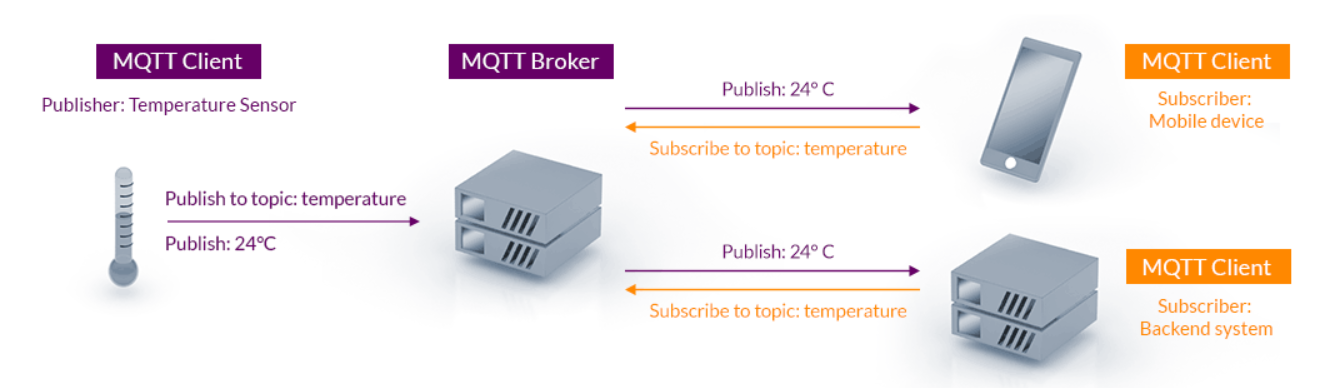
\includegraphics[width=0.8\textwidth]{figures/mqtt-example.png}
    \caption{Esempio di comunicazione tramite MQTT}
    \label{fig:mqtt-example}
\end{figure}

Nel modello publish-subscribe di \ac{MQTT} i dispositivi si dividono in due ruoli principali:
 i publisher, che inviano i messaggi su specifici topic, e i subscriber, che si iscrivono a questi topic per ricevere i messaggi pertinenti. 
 Questo approccio consente una comunicazione flessibile e scalabile, in cui i dispositivi possono interagire in modo dinamico senza la necessità
 di conoscere direttamente gli indirizzi dei destinatari.

Il protocollo \ac{MQTT} è composto da molteplici entità di due tipologie: un singolo broker di messaggi e un numero variabile di client. Il broker \ac{MQTT} è un server 
con la funzione di ricevere i messaggi da tutti i client e di instradarli verso i destinatari interessati. Un client \ac{MQTT} è un qualsiasi dispositivo che esegue una libreria 
\ac{MQTT} e si connette a un broker \ac{MQTT} e può svolgere sia il ruolo di publisher che di subscriber. Quando un publisher ha nuovi dati da trasmettere, 
invia un messaggio con i dati al broker a cui è connesso. Il broker, quindi, distribuisce le informazioni a tutti i client che si sono iscritti a quell’argomento. 
Non è necessario che il publisher conosca il numero o la posizione degli iscritti e questi ultimi, a loro volta, non necessitano di alcuna informazione sui publisher.

Un aspetto cruciale del protocollo \ac{MQTT} è la sua capacità di mantenere aperte le connessioni tra i dispositivi per lunghi periodi, riducendo al minimo la latenza 
e ottimizzando l'efficienza della comunicazione. Questo risulta particolarmente importante in contesti dove è essenziale uno scambio continuo e tempestivo di dati 
in tempo reale, permettendo un monitoraggio costante e affidabile. Tale caratteristica rende \ac{MQTT} ideale per applicazioni che richiedono una trasmissione dati 
ininterrotta e reattiva, garantendo prestazioni ottimali anche in ambienti con risorse limitate e connettività intermittente.

I principali tipi di messaggi \ac{MQTT} sono quattro:
\begin{itemize}
    \item \textbf{Connect}: il client attende che venga stabilita una connessione con il broker e crea un collegamento tra i nodi;
    \item \textbf{Disconnect}: attende se il client \ac{MQTT} deve terminare delle operazioni e poi chiude la sessione TCP/IP;
    \item \textbf{Publish}: il client pubblica un messaggio nella classe specificato;
    \item \textbf{Subscribe}: iscrive il client all’argomento specificato;
\end{itemize}

\subsection{Formato pacchetti MQTT}
Un pacchetto \ac{MQTT} è composto da diverse parti strutturate in modo specifico, può essere suddiviso nelle seguenti componenti principali:

\begin{figure}[H]
    \centering
    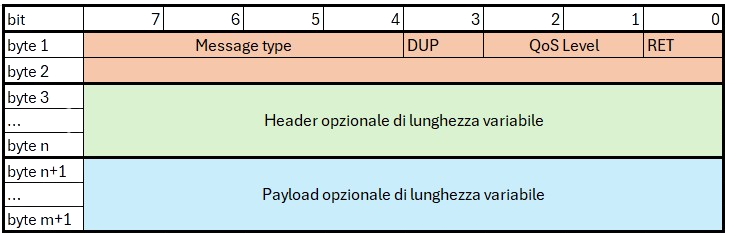
\includegraphics[width=0.8\textwidth]{figures/mqtt-packet.png}
    \caption{formato di un pacchetto MQTT}
    \label{fig:mqtt-packet}
\end{figure}

\begin{itemize}
\item \textbf{Fixed Header (Intestazione Fissa):} Ogni pacchetto \ac{MQTT} contiene un'intestazione fissa che è obbligatoria e ha una lunghezza di 2 byte. 
L'intestazione fissa include il tipo di messaggio, il livello di \ac{QoS}, la lunghezza rimanente del pacchetto e informazioni sui flag di controllo
tra cui DUP (duplicate) che indica se è il primo tentativo di invio di tale pacchetto e RET (retain) che indica se tale pacchetto deve essere salvato nel server.
I tipi di messaggio possono includere CONNECT, PUBLISH, SUBSCRIBE, UNSUBSCRIBE, DISCONNECT.
\item \textbf{Variable Header (Intestazione Variabile):} L'intestazione variabile è opzionale e viene utilizzata in base al tipo di pacchetto. 
Questa sezione può includere diversi campi come l'identificatore del pacchetto, i codici di ritorno e altre informazioni specifiche del tipo di messaggio. 
Ad esempio, nei pacchetti di tipo PUBLISH, l'intestazione variabile include il topic del messaggio.
\item \textbf{Payload (Corpo del Messaggio):} Il corpo del messaggio o payload è anch'esso opzionale e contiene i dati effettivi da trasmettere. 
La lunghezza del payload può variare e nei pacchetti PUBLISH, esso contiene il contenuto del messaggio che viene inviato agli abbonati al topic specifico. 
La presenza e il contenuto del payload dipendono dal tipo di messaggio specifico.
\end{itemize}

\subsection{Quality of Service (QoS)}

\ac{MQTT} offre funzionalità avanzate per la gestione delle connessioni, la sicurezza e la qualità del servizio (\ac{QoS}), che consentono di personalizzare e ottimizzare 
la comunicazione in base alle esigenze specifiche dell'applicazione. Queste caratteristiche lo rendono un protocollo estremamente flessibile e adattabile, 
in grado di soddisfare una vasta gamma di requisiti e casi d'uso nell'ambito dell'\ac{IoT}. 
Ogni livello di \ac{QoS} in \ac{MQTT} offre un trade-off tra affidabilità e overhead di rete, permettendo agli sviluppatori di scegliere il livello più appropriato in base alle esigenze 
specifiche dell'applicazione, semplicemente modificando il valore dei due bit che indicano il livello \ac{QoS} nei pachetti, tramite le API fornite dalle librerie. 

\begin{figure}[H]
    \centering
    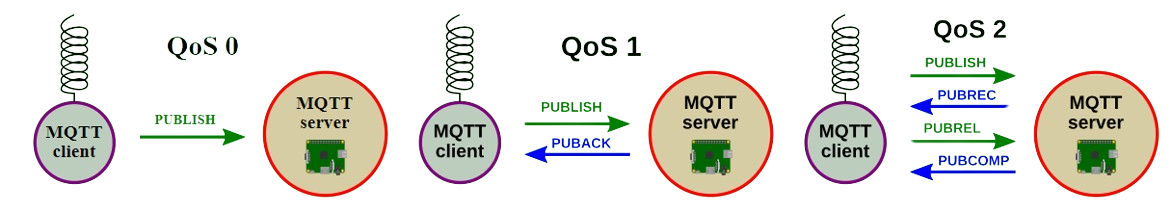
\includegraphics[width=0.8\textwidth]{figures/mqtt-qos.png}
    \caption{funzionamento dei diversi livelli di QoS}
    \label{fig:mqtt-qos}
\end{figure}

Il livello di \ac{QoS} 0, noto anche come `al massimo una volta' (at most once), garantisce che i messaggi vengano inviati senza conferma di ricezione. 
I messaggi vengono consegnati in modo best effort, il che significa che non ci sono garanzie di consegna. Questo livello di \ac{QoS} è utilizzato quando la perdita 
di messaggi occasionali è accettabile, come nelle applicazioni dove la latenza è più importante dell'affidabilità, ad esempio per il monitoraggio di dati in tempo reale 
che vengono aggiornati frequentemente.

Il livello di \ac{QoS} 1, noto anche come `almeno una volta' (at least once), garantisce che i messaggi vengano consegnati almeno una volta al destinatario. Ciò implica 
che il mittente continua a inviare il messaggio finché non riceve una conferma di ricezione (acknowledgement) dal destinatario. Tuttavia, questo può portare alla possibilità 
di ricevere duplicati del messaggio. Il livello \ac{QoS} 1 è utilizzato quando è importante che i messaggi vengano ricevuti, anche se ciò significa ricevere duplicati, 
ad esempio per le transazioni di dati critici che devono essere garantite.

Il livello di \ac{QoS} 2, noto anche come `esattamente una volta' (exactly once), garantisce che ogni messaggio venga consegnato esattamente una volta al destinatario. 
Questo livello di \ac{QoS} utilizza un meccanismo di handshake a quattro fasi per assicurare che i messaggi non vengano duplicati e non vadano persi, garantendo la massima 
affidabilità. Questo livello di \ac{QoS} è utilizzato in scenari dove è fondamentale evitare duplicati e garantire la consegna esatta di ogni messaggio, come nelle applicazioni 
finanziarie o nei sistemi di controllo industriale.

\pagebreak %avoids first 2 line of next subsection to be at the bottom of the page
\subsection{MQTT over WebSocket}

\ac{MQTT} over WebSocket rappresenta una combinazione potente che estende le capacità del protocollo \ac{MQTT} nel contesto delle applicazioni web. WebSocket è un protocollo 
di comunicazione che fornisce un canale full-duplex su una singola connessione \ac{TCP}, consentendo una comunicazione bidirezionale in tempo reale tra il client e il server.

L'integrazione di \ac{MQTT} con WebSocket permette ai client basati su web di comunicare direttamente con un broker \ac{MQTT}, eliminando la necessità di intermediari o di 
soluzioni di polling inefficaci. Questo è particolarmente utile per le applicazioni \ac{IoT} che richiedono aggiornamenti in tempo reale e un'interazione continua tra 
dispositivi e interfacce utente basate su web. Le principali caratteristiche di \ac{MQTT} over WebSocket includono:

\begin{itemize}
    \item \textbf{Compatibilità Browser}: 
    Consente ai browser web di stabilire connessioni \ac{MQTT} direttamente, facilitando lo sviluppo di applicazioni web interattive e in tempo reale.
    \item \textbf{Efficienza della Connessione}: 
    Utilizza una singola connessione \ac{TCP} per gestire sia il canale di comunicazione \ac{MQTT} che la trasmissione dei dati, riducendo il sovraccarico di rete.
    \item \textbf{Sicurezza}: 
    Supporta la crittografia SSL/TLS per garantire che la comunicazione tra il client e il server sia sicura, proteggendo i dati trasmessi da intercettazioni e attacchi.
    \item \textbf{Flessibilità}: 
    Permette una facile integrazione con le infrastrutture web esistenti, utilizzando lo stesso stack di tecnologia web e riducendo la complessità del sistema.
\end{itemize}

\ac{MQTT} over WebSocket è ideale per le applicazioni che necessitano di aggiornamenti frequenti e rapidi, come dashboard di monitoraggio, sistemi di allarme in tempo reale, 
e applicazioni di controllo remoto. La combinazione di \ac{MQTT} e WebSocket offre una soluzione robusta e scalabile per la comunicazione in tempo reale nel mondo dell'\ac{IoT}.

\section{Dependency Injection}

Nel contesto dell'ingegneria del software, la \textit{Dependency Injection} rappresenta un pattern di progettazione fondamentale per la gestione
 delle dipendenze tra i vari componenti di un sistema. Questo approccio promuove un'architettura modulare e facilita la manutenzione, il testing e l'estensibilità del software.

La Dependency Injection è una tecnica attraverso la quale un oggetto (il \textit{client}) riceve le proprie dipendenze da un oggetto esterno 
(l' \textit{injector}), anziché crearle autonomamente. Le dipendenze sono componenti di cui il client ha bisogno per eseguire le proprie funzionalità.
 In altre parole, la Dependency Injection inverte il controllo della creazione delle dipendenze, trasferendo questa responsabilità a un container o a un framework.

Esistono tre principali varianti di Dependency Injection:
\begin{itemize}
\item \textbf{Constructor Injection}: Le dipendenze vengono fornite tramite il costruttore dell'oggetto. 
    Questo metodo garantisce che le dipendenze siano disponibili al momento della creazione dell'oggetto.
\item \textbf{Setter Injection}: Le dipendenze vengono fornite tramite metodi setter. 
    Questo approccio consente una maggiore flessibilità nella configurazione delle dipendenze dopo la creazione dell'oggetto.
\item \textbf{Interface Injection}: L'oggetto client espone un'interfaccia che permette al container di fornire le dipendenze. 
    Questo metodo è meno comune ma può essere utile in contesti specifici.
\end{itemize}

L'adozione della Dependency Injection offre numerosi vantaggi, tra cui:
\begin{itemize}
    \item \textbf{Maggiore modularità}: I componenti del sistema possono essere sviluppati e testati in isolamento, migliorando la coesione e riducendo l'accoppiamento.
    \item \textbf{Facilità di testing}: Le dipendenze possono essere sostituite con mock o stub, semplificando il processo di unit testing.
    \item \textbf{Manutenzione e estensibilità migliorate}: La separazione delle preoccupazioni facilita la modifica e l'estensione delle funzionalità del sistema
     senza impattare sul resto del codice.
    \item \textbf{Inversione del controllo}: La Dependency Injection implementa il principio di inversione del controllo,
     permettendo al framework di gestire il ciclo di vita degli oggetti e le loro dipendenze.
\end{itemize}

Diversi framework e container sono stati sviluppati per supportare la Dependency Injection in vari linguaggi di programmazione. Un esempio prominente, 
 in particolare per l'ecosistema Kotlin, è \textbf{Koin}: un framework di Dependency Injection per Kotlin che si distingue per la sua semplicità e leggerezza. 
 Koin utilizza una DSL (Domain Specific Language) per definire le dipendenze in modo chiaro e conciso, rendendo l'integrazione e la configurazione estremamente intuitive.
 Koin è particolarmente apprezzato nell'ambito dello sviluppo di applicazioni Android.

La Dependency Injection è un pattern di progettazione che offre una soluzione elegante alla gestione delle dipendenze in sistemi software complessi.
 La sua adozione consente di sviluppare applicazioni modulari, testabili e facilmente manutenibili, contribuendo a migliorare la qualità complessiva del software.
 Nelle sezioni successive, esploreremo più in dettaglio i vari aspetti della Dependency Injection, i suoi benefici e come implementarla efficacemente utilizzando diversi framework,
 con un focus particolare su Koin per applicazioni Kotlin.
    
 \section{PulvReAKt}
PulvReAKt è un framework leggero e multipiattaforma per Kotlin, progettato per facilitare la pulverizzazione dei sistemi, ovvero la suddivisione di applicazioni complesse
 in muyltemplici componenti modulari che possono essere distribuiti su diverse piattaforme. Il framework supporta \ac{JVM}, \ac{JS} e alcune piattaforme native, come Linux, macOS e iOS. 
 PulvReAKt consente di definire, configurare e distribuire componenti software utilizzando protocolli di comunicazione come \ac{MQTT} e RabbitMQ, rendendolo particolarmente adatto 
 per lo sviluppo di applicazioni distribuite e sistemi \ac{IoT}. Consente di suddividere l'applicazione in componenti indipendenti, facilitando lo sviluppo e la manutenzione. 
 Supporta \ac{JVM}, \ac{JS} e varie piattaforme native, permettendo l'esecuzione dei componenti in diversi ambienti.
 
\section{Kotlin}
La scelta del linguaggio utilizzato per questo progetto è stata relativamente semplice, poiché il progetto PulvReAKt, nel quale è contestualizzato, 
è scritto interamente in Kotlin con target Multiplatform. La maggior parte dello sviluppo è stata eseguita in Kotlin, con l'unica eccezione dell'utilizzo di una libreria 
JavaScript per lo sviluppo della parte \ac{JS}, integrata comunque all'interno di Kotlin grazie alla sua interoperabilità.

Kotlin è un linguaggio di programmazione moderno sviluppato da JetBrains, noto per il suo approccio pragmatico e la sua forte interoperabilità con Java. 
Dal suo lancio nel 2011, Kotlin ha guadagnato rapidamente popolarità, diventando nel 2017 il linguaggio ufficiale per lo sviluppo di applicazioni Android. 

Kotlin è stato progettato per essere conciso, riducendo la quantità di codice boilerplate necessario. Grazie alle funzioni lambda e alle estensioni di funzioni, 
il codice scritto in Kotlin risulta più leggibile e mantenibile rispetto a Java. Inoltre, Kotlin si propone di minimizzare gli errori a runtime, 
spostando la rilevazione degli errori al tempo di compilazione.

Uno dei punti di forza di Kotlin è la sua totale interoperabilità con Java. Questo significa che il codice Kotlin può chiamare ed essere chiamato da codice Java senza difficoltà. 
Questo facilita la migrazione graduale da Java a Kotlin nei progetti esistenti, permettendo agli sviluppatori di integrare Kotlin in maniera incrementale.

Kotlin introduce le coroutines, una potente astrazione per la programmazione asincrona e concorrente. Le coroutines offrono un modo semplice ed efficiente per gestire operazioni
che altrimenti richiederebbero la gestione complessa dei thread. Esse permettono di scrivere codice asincrono in uno stile sequenziale, migliorando la leggibilità e
riducendo il rischio di errori.

Le coroutines in Kotlin sono supportate a livello di linguaggio, con una libreria standard che fornisce molte funzionalità pronte all'uso. 
Ecco alcuni dei principali vantaggi delle coroutines:

\begin{itemize}
    \item \textbf{Semplicità del codice asincrono:} Le coroutines permettono di scrivere codice che sembra sincrono ma che viene eseguito in modo asincrono, 
    semplificando notevolmente la gestione delle operazioni I/O e altre operazioni bloccanti.
    \item \textbf{Efficienza delle risorse:} Le coroutines sono molto leggere rispetto ai thread tradizionali. Possono essere sospese e riprese senza un costo significativo, 
    consentendo una gestione efficiente delle risorse.
    \item \textbf{Facilità di cancellazione:} Le coroutines forniscono meccanismi per gestire la cancellazione delle operazioni in corso, 
    riducendo il rischio di risorse bloccate o perdite di memoria.
    \item \textbf{Composizione semplice:} Le coroutines permettono di comporre in modo semplice operazioni asincrone, rendendo il codice più modulare e facile da mantenere.
\end{itemize}

L'utilizzo delle coroutines in Kotlin rappresenta un approccio moderno alla programmazione concorrente, 
semplificando notevolmente il processo di scrittura e gestione del codice asincrono.

La sintassi concisa e le caratteristiche avanzate di Kotlin contribuiscono ad aumentare la produttività degli sviluppatori. 
Funzionalità come le funzioni di estensione, la gestione avanzata delle nullità e le espressioni lambda riducono il codice boilerplate e semplificano lo sviluppo, 
permettendo agli sviluppatori di concentrarsi sulla logica applicativa piuttosto che sui dettagli implementativi.

La forte tipizzazione e le funzionalità di sicurezza integrata di Kotlin contribuiscono a migliorare la qualità del codice. 
Il compilatore di Kotlin è in grado di rilevare molti tipi di errori a tempo di compilazione, riducendo il numero di bug presenti nel software finito. Inoltre, 
la gestione avanzata delle nullità e le funzioni di estensione aiutano a scrivere codice più robusto e meno incline agli errori.

Uno degli aspetti più potenti di Kotlin è la sua capacità di supportare lo sviluppo multiplatform. Grazie al quale gli sviluppatori possono scrivere 
un unico set di codice Kotlin che può essere condiviso e utilizzato su diverse piattaforme, come la \ac{JVM}, JavaScript e la compilazione nativa. 
Questo approccio consente agli sviluppatori di massimizzare la condivisione del codice, riducendo al minimo la duplicazione e semplificando la manutenzione dell'applicazione 
su più piattaforme.

\chapter{Requisiti}\label{chap:Requisiti}

\section{Requisiti funzionali}

Il progetto si propone di offrire un gestore delle comunicazioni versatile, capace di adattarsi a diversi ambiti applicativi. 
In particolare, è stato progettato pensando alle funzionalità richieste da un sistema distribuito ed eterogeneo come PulvReAKt, nel quale è stato successivamente integrato. 
PulvReAKt è caratterizzato dalla possibilità di avere componenti dislocate in posizioni geografiche diverse, con capacità e risorse variabili. 
Questo sistema deve essere quindi in grado di operare efficacemente in contesti molto diversificati, incluso l'ambito \ac{IoT}, dove le macchine coinvolte dispongono 
spesso di risorse hardware limitate. Inoltre, il sistema deve essere progettato per funzionare correttamente anche in ambienti con connettività di rete instabile o variabile, 
garantendo prestazioni adeguate indipendentemente dalle condizioni di rete.

Uno degli obiettivi principali del progetto è assicurare che le comunicazioni avvengano in modo efficiente e affidabile. Particolare attenzione è stata posta nel garantire 
che i messaggi vengano recapitati esclusivamente ai destinatari interessati. Questo richiede l'implementazione di meccanismi sofisticati di gestione dei messaggi, 
che consentano un indirizzamento preciso e prevengano lo spreco di risorse. La capacità di indirizzare correttamente i messaggi è fondamentale per evitare sovraccarichi 
di rete e per mantenere l'integrità e la sicurezza delle comunicazioni.

La gestione dei canali di comunicazione deve essere trasparente per l'utente finale. Tuttavia, è responsabilità dell'utente definire quali entità debbano comunicare
tra loro, definire un formato per i messaggi e conseguentemente formattarli correttamente, poiché il sistema è progettato per ricevere il messaggio in input, 
insieme alle entità sorgente e destinazione, e per inviarlo al destinatario corretto mantenendo l'integrità del mittente e del contenuto del messaggio. 
La formattazione non sarà unificata, se non per quanto riguarda l'incapsulamento necessario per garantire l'invio e la ricezione corretti dei messaggi, utilizzando \ac{MQTT}.

Un ulteriore aspetto critico del progetto è la necessità di sviluppare test esaustivi. La scrittura di test approfonditi è fondamentale per garantire la robustezza 
e l'affidabilità del sistema. I test devono coprire un'ampia gamma di scenari, inclusi quelli più comuni e quelli meno frequenti ma potenzialmente problematici. 
È essenziale che vengano testati tutti i possibili casi d'uso, compresi quelli che coinvolgono condizioni di rete instabili, errori di comunicazione e gestione 
delle risorse limitate. I test devono inoltre verificare che il sistema risponda correttamente a input non validi e che mantenga l'integrità dei dati durante 
l'intero processo di comunicazione. Solo attraverso una rigorosa attività di testing è possibile assicurare che il sistema soddisfi i requisiti funzionali e 
operi come atteso in tutte le casistiche di utilizzo.

\section{Scalabilità}

Il modulo di comunicazione progettato per utilizzare \ac{MQTT}, deve essere in grado di scalare efficacemente per gestire un numero variabile 
di entità comunicanti, sia che esse siano poche o molte, sia che queste comunichino spesso o raramente.

Il sistema deve essere modulare per facilitare l'aggiunta o la rimozione di componenti senza compromettere il funzionamento generale. 
Utilizzando \ac{MQTT} come middleware per la comunicazione asincrona, deve garantire la capacità di scalare orizzontalmente. 
È essenziale che il protocollo di comunicazione sia leggero e ad alte prestazioni, permettendo di gestire un elevato numero di connessioni simultanee 
con un overhead minimo. Per ottimizzare l'uso delle risorse di rete, deve essere supportato il multiplexing, che consente di gestire più connessioni 
su un singolo canale di comunicazione.

Per quanto riguarda la gestione delle connessioni, il sistema deve mantenere connessioni persistenti per ridurre il costo di stabilire connessioni multiple. 
Inoltre, deve utilizzare un pool di connessioni per riutilizzare connessioni esistenti, migliorando così l'efficienza complessiva del sistema. 
La gestione efficiente delle connessioni è cruciale per assicurare che il sistema possa gestire un numero crescente di entità comunicanti senza degradare le prestazioni.

Un altro aspetto fondamentale per la scalabilità è la gestione della coda di messaggi. Il sistema deve utilizzare code di messaggi distribuite per gestire efficacemente 
l'accodamento e la distribuzione dei messaggi tra le varie entità. Questo approccio garantisce che il sistema possa scalare in modo lineare con l'aumento del numero 
di messaggi e delle entità coinvolte, mantenendo alta la performance e l'affidabilità.

Questi requisiti sono necessari per assicurare che il modulo di comunicazione sia in grado di operare in modo efficiente e affidabile, 
indipendentemente dal numero di entità coinvolte e dalle condizioni di rete. Mantenendo alte prestazioni e stabilità del sistema, si garantisce che le comunicazioni 
avvengano in modo fluido e continuo, soddisfacendo le esigenze di un ambiente di rete variabile e potenzialmente instabile.

\section{Affidabilità}

Un aspetto cruciale nella comunicazione tra i componenti di un sistema distribuito è la robustezza e l'affidabilità, elementi fondamentali per garantire 
il corretto funzionamento complessivo del sistema. I componenti devono essere in grado di inviare e ricevere messaggi utilizzando il protocollo \ac{MQTT}. 
Questo richiede l'integrazione di librerie specifiche per \ac{MQTT}, assicurando che i messaggi possano essere formattati, inviati e ricevuti correttamente. 
È imperativo garantire l'affidabilità nella consegna dei messaggi, assicurando in alcuni casi che ogni messaggio venga ricevuto dal destinatario previsto. 
Per raggiungere questo obiettivo, è necessario implementare la gestione delle conferme di ricezione, meccanismi di ritrasmissione in caso di fallimento e 
gestione delle code di messaggi per evitare perdite.

Il progetto offre questa possibilità utilizzando una \ac{QoS} di livello 1 o 2, permettendo allo sviluppatore di scegliere di utilizzare tali garanzie di ricezione 
e non duplicazione.Il progetto offre anche la possibilità di usare \ac{QoS} 0 e quindi non garantire la consegna, ma consente avere prestazioni più elevate, 
in particolare su dispositivi \ac{IoT} dotati di scarsa poternza hardware.

La gestione delle code di messaggi rappresenta un'altra componente critica. Un sistema di coda ben progettato può aiutare a prevenire la perdita di messaggi in 
situazioni di traffico elevato o in caso di disconnessioni temporanee. Implementare meccanismi di bufferizzazione e di ritrasmissione può migliorare significativamente 
l'affidabilità complessiva del sistema. In particolare, le code devono essere in grado di gestire i picchi di traffico senza perdere dati e devono poter recuperare 
rapidamente in caso di disconnessione, assicurando che i messaggi vengano consegnati non appena la connessione viene ristabilita.

Il modulo di comunicazione deve includere funzionalità di logging e monitoraggio per tracciare l'attività e le performance del sistema. Questi strumenti permettono 
di identificare e risolvere rapidamente eventuali problemi, migliorando la reattività del sistema alle condizioni di errore. Il logging dettagliato degli eventi di 
comunicazione aiuta anche nella diagnosi e nella prevenzione di guasti futuri, fornendo dati preziosi per l'analisi delle cause principali dei problemi. 
Un sistema di monitoraggio efficiente può allertare gli operatori in caso di anomalie, permettendo interventi tempestivi e mirati per minimizzare l'impatto sugli utenti finali.

L'affidabilità può essere ulteriormente migliorata attraverso l'adozione di pratiche DevOps, con pipeline \ac{CI/CD}, che assicurano che le nuove versioni del software 
vengano distribuite in modo sicuro e senza interruzioni, mantenendo un elevato standard di qualità e affidabilità. La continua integrazione e distribuzione permette di 
rilevare e risolvere rapidamente i bug, riducendo al minimo il rischio di errori introdotti da nuove funzionalità o aggiornamenti. Queste pratiche, combinate con tecniche 
di testing rigorose come i test di stress e i test di carico, valutano le prestazioni del sistema sotto condizioni estreme, identificando i punti deboli del sistema e 
apportando le necessarie migliorie prima che i problemi si manifestino in produzione.

\section{Interoperabilità}

L'interoperabilità si riferisce alla capacità dei diversi sistemi e componenti software di lavorare insieme senza problemi, scambiando dati e utilizzando le informazioni scambiate 
in modo efficace. Nel contesto di PulvReAKt, questo significa che i componenti sviluppati per \ac{JVM} devono poter interagire con quelli sviluppati in JavaScript o con quelli 
che girano su piattaforme native. Questo richiede che il protocollo di comunicazione, in questo caso \ac{MQTT}, sia implementato in modo standard e conforme su tutte le piattaforme.
\subsection{Java Virtual Machine}

La \ac{JVM} è una macchina virtuale che esegue bytecode Java, ed è la piattaforma di riferimento per lo sviluppo in Java e Kotlin. 
Essa offre una serie di caratteristiche che la rendono una scelta popolare per l'implementazione di applicazioni complesse e ad alte prestazioni.
Le caratteristiche principali della \ac{JVM} sono:

\begin{itemize}
\item \textbf{Interoperabilità}: La \ac{JVM} permette l'interoperabilità tra Kotlin e Java, consentendo l'uso di librerie e strumenti Java consolidati, 
 permettendo agli sviluppatori di sfruttare l'ampio ecosistema Java esistente.
\item \textbf{Portabilità}: Il bytecode generato può essere eseguito su qualsiasi dispositivo dotato di una \ac{JVM}, garantendo portabilità cross-platform. 
Questo è particolarmente utile per le applicazioni distribuite su una vasta gamma di dispositivi e sistemi operativi.
\item \textbf{Ottimizzazioni di Runtime}: La \ac{JVM} include un Just-In-Time (JIT) compiler che ottimizza il codice durante l'esecuzione, migliorando le performance e 
consentendo un'esecuzione più veloce delle applicazioni Kotlin rispetto a linguaggi interpretati o compilati staticamente.
\item \textbf{Garbage Collection}: Gestione automatica della memoria tramite garbage collection, riducendo il rischio di memory leaks. 
Allevia gli sviluppatori dalla necessità di gestire manualmente l'allocazione e la deallocazione della memoria, semplificando lo sviluppo e riducendo il rischio di errori.
\end{itemize}

\subsection{JavaScript e Node.js}

JavaScript è il linguaggio di scripting dominante per lo sviluppo web client-side, eseguito all'interno dei browser. Kotlin/\ac{JS} permette di compilare codice Kotlin in JavaScript, 
sfruttando le capacità di questa piattaforma. Le caratteristiche principali di \ac{JS} sono:

\begin{itemize}
\item \textbf{Compatibilità con il Web}: JavaScript è nativamente supportato dai browser, permettendo l'esecuzione di applicazioni Kotlin/\ac{JS} direttamente nel contesto web e 
consente agli sviluppatori di creare applicazioni web interattive e dinamiche utilizzando Kotlin come linguaggio di sviluppo.
\item \textbf{Ecosistema di Librerie}: Ampia disponibilità di librerie e framework per lo sviluppo web, che possono essere utilizzati anche con Kotlin/\ac{JS}. 
Include librerie per la gestione del DOM\footnote{
    DOM (Document Object Model): Rappresentazione ad albero di un documento HTML/XML che permette di accedere e modificare dinamicamente la struttura e 
    il contenuto delle pagine web.
}, l'interazione con API REST\footnote{
    API REST (Representational State Transfer): Insieme di convenzioni per creare servizi web che permettono la comunicazione 
    tra client e server utilizzando operazioni HTTP standard.
}, la manipolazione dei dati JSON\footnote{
    JSON (JavaScript Object Notation): Formato di testo leggero per lo scambio di dati, facilmente leggibile dagli umani e parsabile dai computer.
} 
e molto altro ancora, consentendo quindi agli sviluppatori di sfruttare le funzionalità esistenti senza doverle implementare nuovamente.
\item \textbf{Asincronia}: Supporto nativo per le operazioni asincrone tramite callback, Promises e async/await che vanno a sopperire alla mancanza di capacità multithread 
essendo progettato per lavorare anche in contesto browser, quindi con un singolo thread. Questa particolarita è estremamente utile per le applicazioni web che devono gestire 
operazioni di rete, come il caricamento di dati da un server remoto.
\item \textbf{Interoperabilità}: Kotlin/\ac{JS} permette l'interoperabilità con le API JavaScript esistenti, facilitando l'integrazione con altre tecnologie web,
consentendo agli sviluppatori di utilizzare librerie e framework JavaScript esistenti all'interno del codice Kotlin, con una maggiore flessibilità 
e libertà di scelta nella progettazione delle applicazioni.
\end{itemize}

\begin{itemize}
\item \textbf{Node.js} rappresenta una potente piattaforma per lo sviluppo backend, estendendo le capacità di JavaScript oltre il browser e offrendo un ambiente efficiente e scalabile 
per la creazione di applicazioni server-side moderne. Utilizzando Node.js, gli sviluppatori possono beneficiare di un ecosistema ricco di strumenti avanzati per costruire
applicazioni robuste e performanti.
\item \textbf{Event-driven e Non-blocking I/O}: Node.js utilizza un modello event-driven e non-blocking per le operazioni di I/O, consentendo di gestire un numero elevato di connessioni
 concorrenti con un singolo thread grazie al meccanismo delle promise in \ac{JS}.
\item \textbf{Ecosistema di Moduli }: Node.js ha un vasto ecosistema di moduli e pacchetti disponibili tramite npm (Node Package Manager). 
Questi moduli coprono una vasta gamma di funzionalità, come la gestione del database, la manipolazione dei file e la creazione di server web. 
\end{itemize}

\subsection{Native}

Kotlin/Native permette di compilare codice Kotlin direttamente in codice macchina eseguibile su dispositivi target, senza la necessità di una macchina virtuale o un interprete.
Le caratteristiche principali delle diverse piattaforme native sono:

\begin{itemize}
\item \textbf{Esecuzione Diretta}: Compilazione in codice nativo che viene eseguito direttamente dall'hardware, senza layer di interpretazione. 
Si traduce in prestazioni superiori rispetto alle applicazioni eseguite su una macchina virtuale o interprete, poiché non vi è alcun overhead dovuto alla traduzione 
del bytecode in istruzioni di macchina.
\item \textbf{Performance}: Le applicazioni native tendono ad avere performance superiori rispetto a quelle eseguite su una macchina virtuale o interprete, 
grazie alla compilazione diretta. Questo è particolarmente importante per le applicazioni ad alte prestazioni che richiedono un tempo di risposta rapido e una bassa latenza.
\item \textbf{Accesso a Funzionalità di Sistema}: Possibilità di accedere direttamente alle API di sistema e alle risorse hardware, offrendo maggior controllo e ottimizzazione. 
Consente agli sviluppatori di creare applicazioni che interagiscono direttamente con l'hardware sottostante, sfruttando appieno le capacità del dispositivo target.
\item \textbf{Assenza di Overhead}: Sebbene Kotlin/Native includa un garbage collector, quando viene eseguito su piattaforme native non vi è nessun overhead dovuto alla 
gestione della macchina virtuale. Questo significa che le risorse del sistema possono essere utilizzate in modo più efficiente, riducendo il consumo di memoria e CPU.
\item \textbf{Cross-platform}: La capacità di supportare diverse piattaforme, inclusi iOS, Windows, Linux e macOS, facilita lo sviluppo di applicazioni multi-piattaforma e 
consente agli sviluppatori di scrivere un'unica base di codice Kotlin che può essere compilato ed eseguito su una varietà di dispositivi e sistemi operativi, 
riducendo al minimo lo sforzo di sviluppo e la complessità del codice.
\end{itemize}

\chapter{Design}\label{chap:Design}

\section{Struttura di MQTT}

La discrepanza tra il modello publish-subscribe caratteristico di \ac{MQTT} e la necessità di comunicazione diretta tra le entità, come previsto dal progetto, richiede una definizione accurata 
della struttura dei topic di \ac{MQTT}. Per affrontare questa sfida, si è deciso di strutturare i topic nella forma \texttt{nomeProgetto/mittente/destinatario}. 
In questa struttura, 'nomeProgetto' rappresenta un topic unico all'interno del progetto, che ospita tutti i topic necessari per la comunicazione tra le singole entità. 
Ad esempio, nel progetto PulvReAKt, il nome del progetto è 'PulvReAKt', ma può essere personalizzato tramite il costruttore del gestore delle comunicazioni.

I componenti 'mittente' e 'destinatario' rappresentano rispettivamente il nome dell'entità che invia il messaggio e quello dell'entità destinataria. 
Questi nomi sono definiti esternamente al modulo comunicativo, rendendo l'utente responsabile della loro unicità all'interno del sistema per evitare ambiguità. 
In alternativa, l'utente può utilizzare nomi comuni per le entità che devono ricevere gli stessi messaggi. Questa struttura permette una gestione chiara e organizzata dei messaggi, 
facilitando il monitoraggio e la manutenzione del sistema di comunicazione.

Si è scelto di utilizzare \ac{MQTT} over WebSocket, dove il pacchetto \ac{MQTT} viene inserito all'interno di un messaggio WebSocket. Questa scelta è motivata principalmente dalla 
maggiore efficienza nell'utilizzo della rete, poiché WebSocket fornisce un canale full-duplex su una singola connessione \ac{TCP}. Questa configurazione permette di gestire sia il 
canale di comunicazione \ac{MQTT} sia la trasmissione dei dati tramite una sola connessione \ac{TCP}, riducendo il sovraccarico di rete e migliorando le prestazioni complessive del sistema, 
garantendo una comunicazione più fluida ed efficiente. La riduzione del sovraccarico è particolarmente importante in ambienti con risorse di rete limitate, 
dove ogni connessione aggiuntiva può influire negativamente sulle prestazioni complessive.

Un altro motivo importante per la scelta di WebSocket è la compatibilità con le infrastrutture HTTP esistenti. WebSocket permette alle comunicazioni \ac{MQTT} di utilizzare strutture HTTP già presenti, 
come la porta HTTP 80, firewall e proxy, che non sarebbero utilizzabili se \ac{MQTT} fosse impiegato direttamente su \ac{TCP}. Questa compatibilità offre vantaggi in termini di sicurezza e gestione della rete, 
facilitando l'integrazione del protocollo \ac{MQTT} in ambienti con restrizioni di rete più rigide.

Per quanto riguarda le caratteristiche dei messaggi inviati e ricevuti, è stato deciso di utilizzare come impostazione predefinita il livello di \ac{QoS} 2 (exactly once), poiché è il livello più affidabile, 
anche se meno efficiente. Tuttavia, si offre all'utente la possibilità di specificare il livello di \ac{QoS} desiderato, 
il valore del ServerKeepAlive (tempo in secondi che il server mantiene la connessione viva dopo l'ultima interazione con il client, impostato di default a 10 secondi) 
e il flag retain del messaggio (che indica se i messaggi inviati vadano salvati in memoria nel broker fino all'arrivo del messaggio successivo, impostato di default a True). 

Il payload dei messaggi è gestito con particolare attenzione: viene inserito nel pacchetto \ac{MQTT} e in quello WebSocket esattamente come ricevuto dall'utente, viene poi inviato al broker e successivamente 
rimosso dal pacchetto \ac{MQTT} per essere restituito all'entità destinataria. Questa gestione assicura che il contenuto del messaggio mantenga la sua integrità e che la comunicazione avvenga in modo trasparente ed efficace, 
rispettando le esigenze di affidabilità e performance del sistema. Questo approccio permette di criptare i messaggi prima dell'invio e decriptarli dopo la ricezione, senza che l'integrità del messaggio venga intaccata dal 
protocollo o dall'utilizzo del progetto.

\section{Struttura delle classi}

\begin{figure}[H]
    \centering
    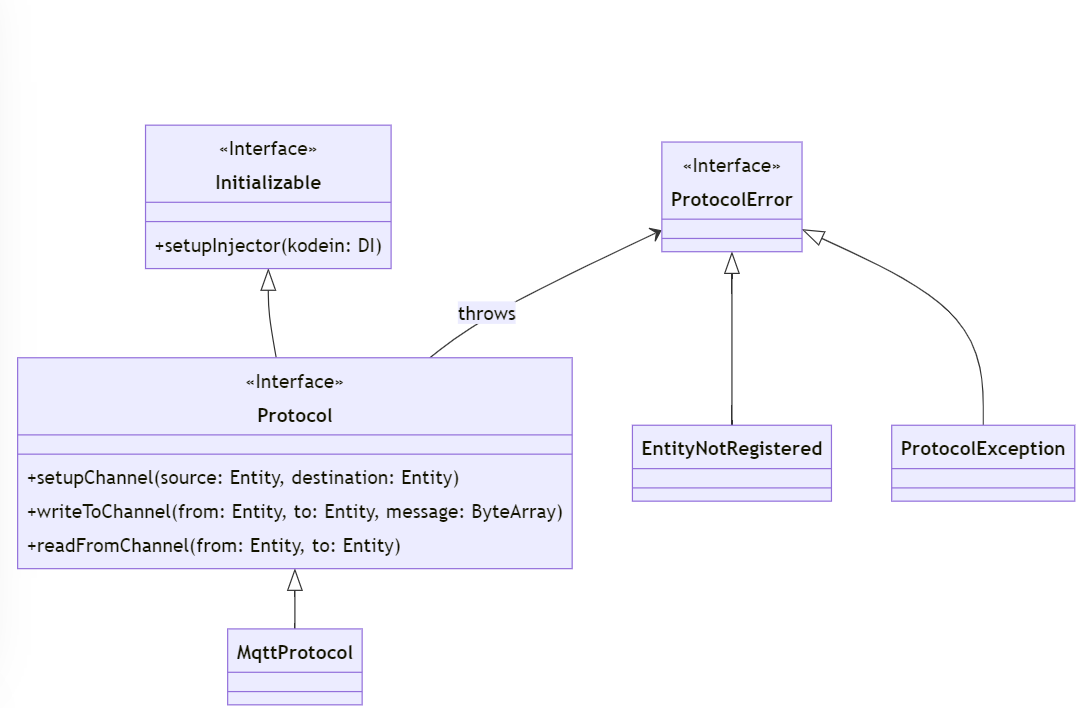
\includegraphics[width=0.8\textwidth]{figures/class-diagram.png}
    \caption{Diagramma delle classi}
    \label{fig:class-diagram}
\end{figure}

Il diagramma delle classi presentato in Figura \ref{fig:class-diagram} illustra l'architettura e le relazioni tra le interfacce e le classi implementate nel progetto. 
Di seguito, viene fornita una descrizione dettagliata di ciascun componente e delle loro interazioni:

\begin{itemize}
    \item \texttt{InjectAwareResource}: è un'interfaccia che definisce il metodo utilizzato per configurare l'iniettore delle dipendenze all'interno di PulvReAKt .

    \item \texttt{ProtocolError}: è un'interfaccia che rappresenta gli errori relativi al protocollo. Viene implementata da due classi concrete:
    \begin{itemize}
        \item \texttt{EntityNotRegistered}: rappresenta un errore che si verifica quando un'entità non è registrata.
        \item \texttt{ProtocolException}: rappresenta un'eccezione generata direttamente dal protocollo \ac{MQTT}, riportata all' interno di Kotlin 
        in modo tale da poterla gestire correttamente e minimizzare gli errori durante l'esecuzione.
    \end{itemize}

    \item \texttt{Protocol}: è un'interfaccia che definisce i metodi essenziali per l'utilizzo di un generico protocollo di comunicazione. 
    Fornisce infatti un metodo per ognuna delle tre operazioni fondamentali:
    \begin{itemize}
        \item \texttt{setupChannel}: metodo per configurare i canali di comunicazione tra due entità \texttt{source} e \texttt{destination}. 
        Nello specifico verrà aperto un canale \texttt{/source/destination} e un canale \texttt{/destination/source}, 
        in quanto ci si aspetta la comunicazione tra le due entità sia bidirezionale nella maggior parte delle casistiche di utilizzo, 
        evitando in questo modo di rendere necessarie due chiamate al metodo, una per direzione di comunicazione nella coppia.
        Una volta chiamato il setup sarà valido per tutto il tempo di esecuzione, sarà quindi sufficiente chiamarlo una volta per ogni coppia 
        \texttt{source} e \texttt{destination}.
        \item \texttt{writeToChannel}: Metodo per scrivere un messaggio al destinatario specificato \texttt{to} rendendo noto il mittente \texttt{from}. 
        Questo metodo può riuscire o fallire con un \texttt{ProtocolError}. Fallisce se il canale di comunicazione tra le entità \texttt{from} e \texttt{to}
        non è stato creato correttamente tramite il metodo \texttt{setupChannel} prima di tentare di mandare un messaggio.
        \item \texttt{readFromChannel}: Metodo per leggere dati dal canale di comunicazione specificato. Questo metodo restituisce un \texttt{Flow} 
        di messaggi che può essere consumato a runtime. Può riuscire o fallire restituendo un \texttt{ProtocolError}. 
        Fallisce se il canale di comunicazione tra le entità \texttt{from} e \texttt{to}
        non è stato creato correttamente tramite il metodo \texttt{setupChannel} prima di tentare di leggere quanto scritto sul canale.
    \end{itemize}

    \item \texttt{MqttProtocol}: Una classe concreta che implementa l'interfaccia \texttt{Protocol}. Questa classe fornisce l'implementazione 
    specifica per il protocollo \ac{MQTT} per le differenti piattaforme, includendo i metodi definiti in \texttt{Protocol}.
    L'implementazione in \texttt{MqttProtocol} sfrutta le funzionalità di \ac{MQTT} per gestire le comunicazioni tra i nodi nel sistema distribuito.

\end{itemize}

\section{Struttura dei Package}
\begin{figure}[H]
    \centering
    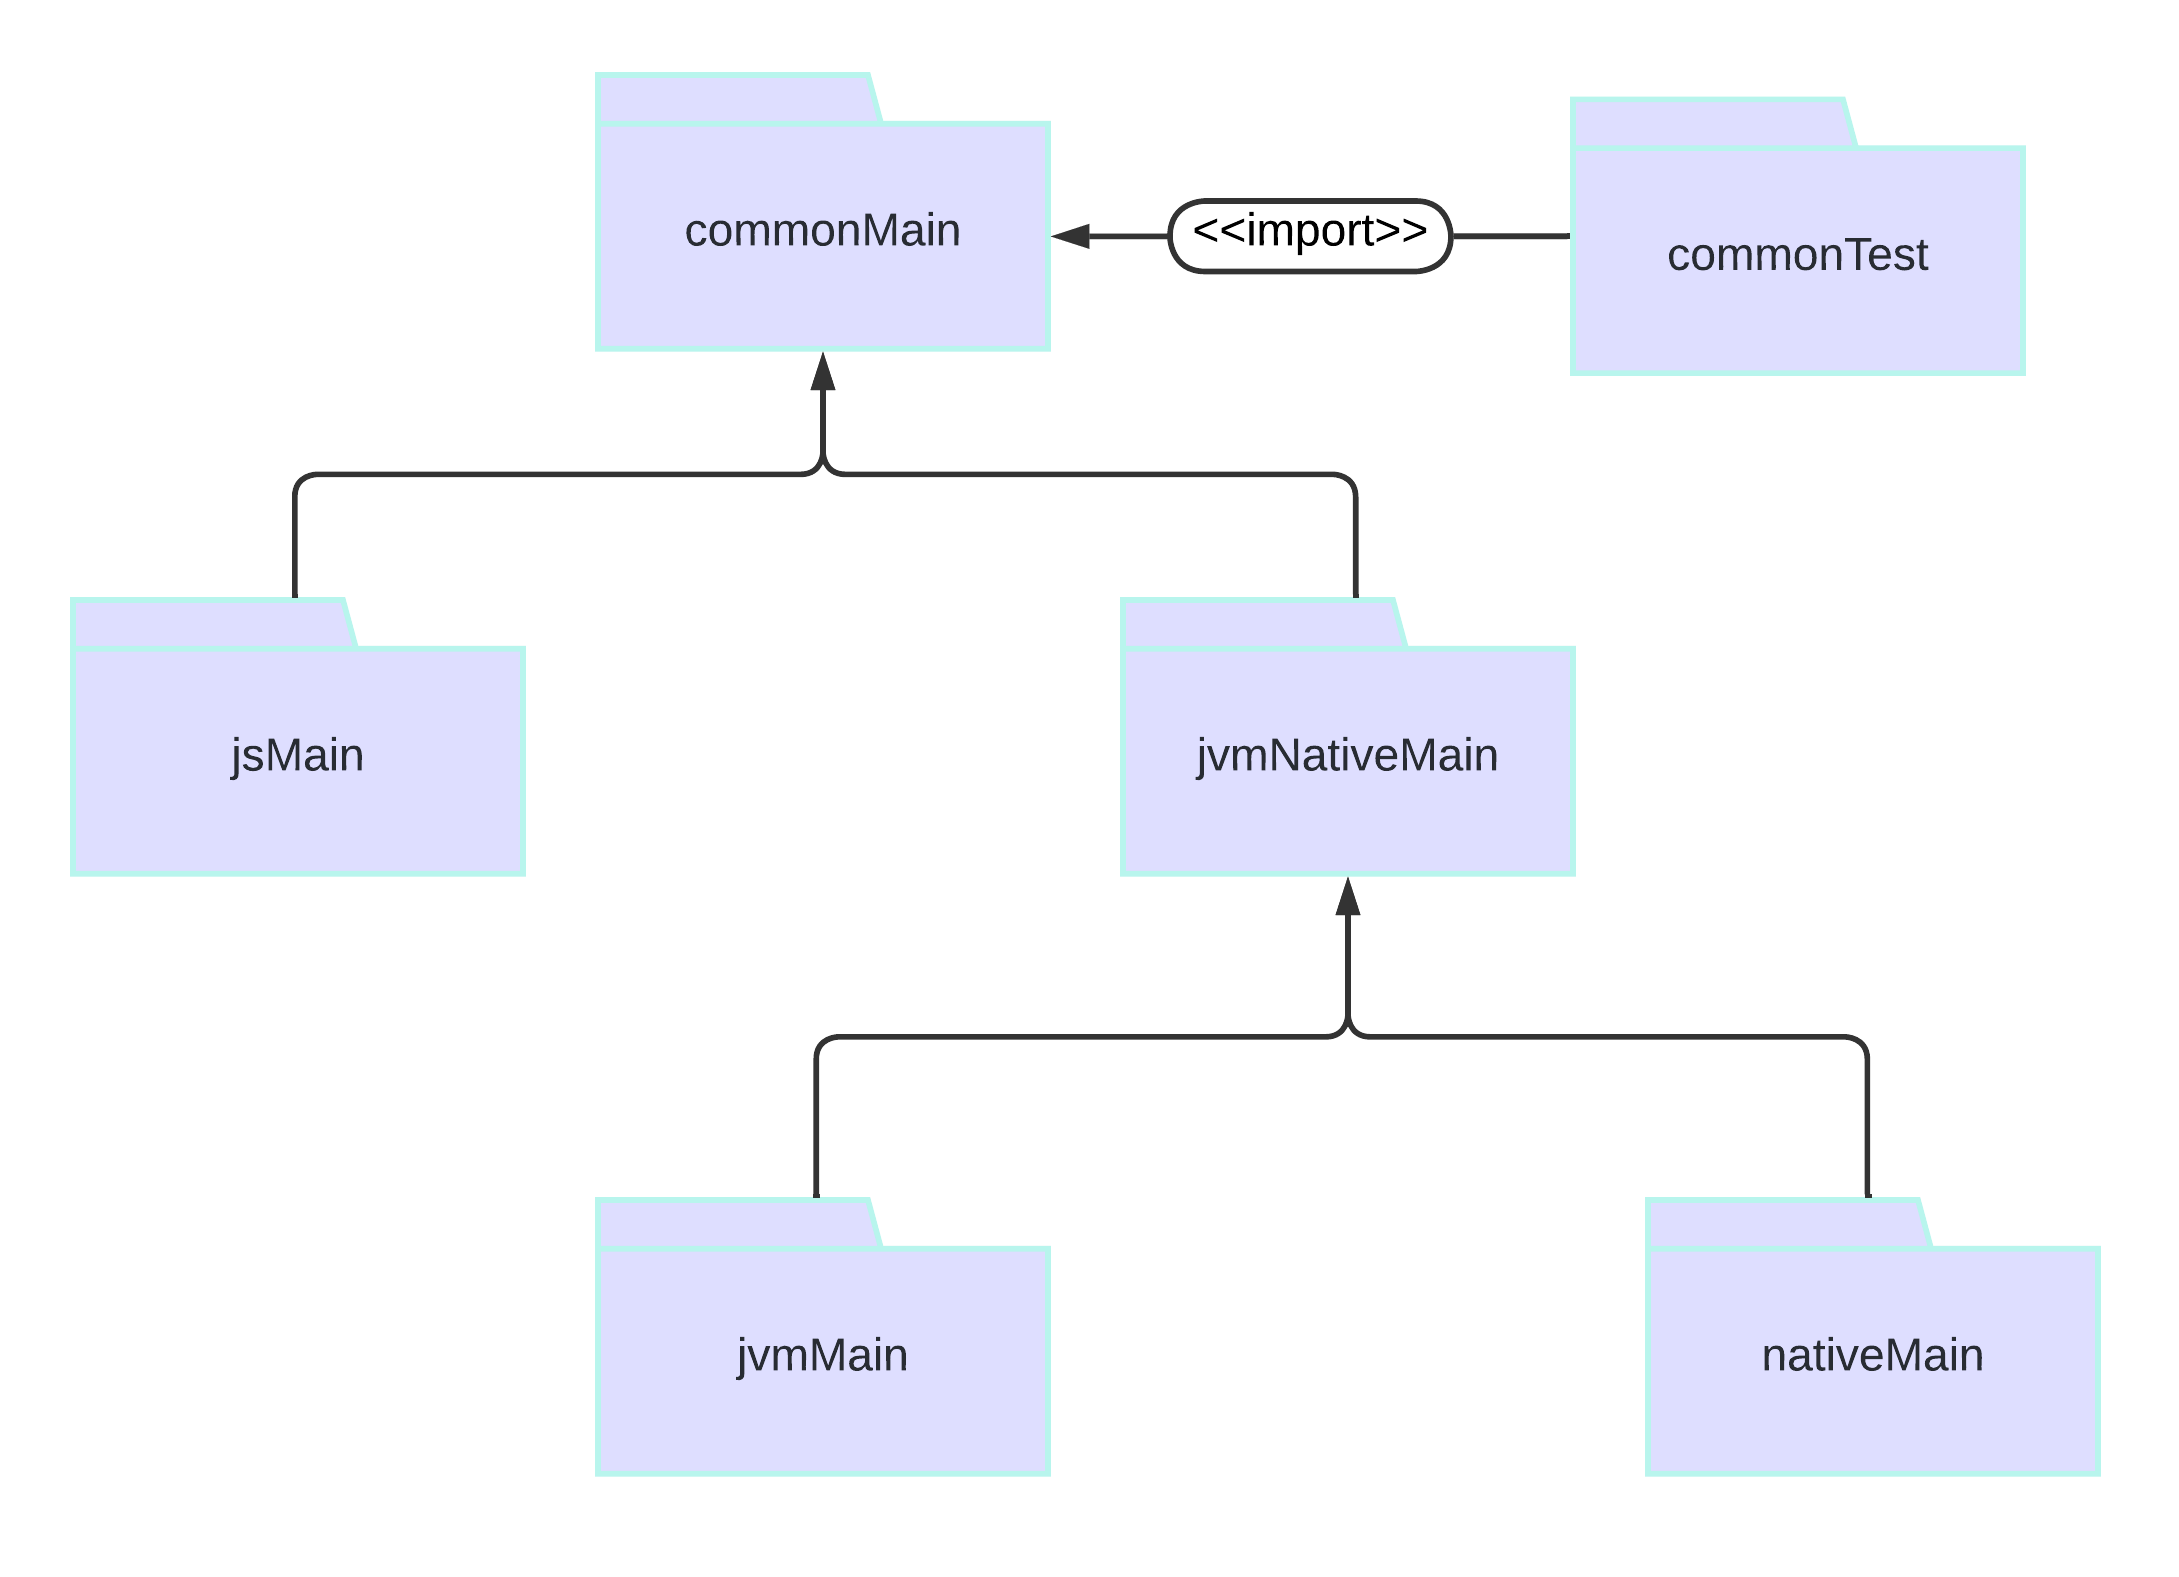
\includegraphics[width=0.8\textwidth]{figures/package-diagram.png}
    \caption{Diagramma dei package}
    \label{fig:diagramma-package}
\end{figure}

Dovendo il progetto funzionare su diverse piattaforme, si è cercato di unificare quanti più target possibili, in modo tale da potere scrivere e revisionare il codice una sola volta.
Si è riusciti ad utilizzare una libreria comune e di conseguenza un modulo unificato per lo sviluppo di \ac{JVM} e native 
mentre, data la natura singlethread di \ac{JS} è stato necessario separare il target dagli altri due. Si è quindi optato per una libreria specifica 
per lo sviluppo con target NodeJS, in modo che questa fosse ottimizzata per l'ambiente specifico. 

Per questo motivo il progetto è stato strutturato in modo tale da avere moduli distinti per ciascun ambiente, con un modulo specifico per \ac{JS} 
e un modulo comune per \ac{JVM} e native. Entrambi questi moduli implementano una API fornita nel modulo comune (\texttt{commonMain}) grazie
alla struttura degli \texttt{expected} e degli \texttt{actual} fornita da Kotlin specificatamente per queste casistiche, in cui le stesse funzionalità
e gli stessi metodi devono essere comuni alle diverse piattaforme ma richiedono implementazioni o librerie sottostanti differenti.

Il modulo comune per la \ac{JVM} e native è chiamato \texttt{jvmNativeMain} e contiene 
un'implementazione comune ai due target. Questo modulo include tutte le funzionalità che possono essere eseguite in un ambiente multithread, 
sfruttando le capacità di concorrenza della \ac{JVM} e delle piattaforme native. In \texttt{jvmNativeMain} sono implementati i componenti core del sistema, 
garantendo che la logica di base sia condivisa e riutilizzabile tra le diverse piattaforme. Questo approccio riduce la duplicazione 
del codice e facilita la manutenzione del progetto.

Dalla struttura di \texttt{jvmNativeMain} dipendono due moduli specifici per ogni target:
\begin{itemize}
    \item \texttt{jvmMain}: Questo modulo estende \texttt{jvmNativeMain} per includere ottimizzazioni e integrazioni necessarie per funzionare efficacemente in un ambiente \ac{JVM}. Qui vengono implementate le funzionalità specifiche che sfruttano le caratteristiche avanzate della \ac{JVM}, come la gestione avanzata dei thread e l'ottimizzazione delle prestazioni.
    \item \texttt{nativeMain}: Questo modulo estende \texttt{jvmNativeMain} per le piattaforme native, includendo le implementazioni necessarie per funzionare su tali ambienti. Viene adattato per sfruttare le peculiarità delle diverse piattaforme native, garantendo efficienza e compatibilità con il codice nativo.
\end{itemize}

Per quanto riguarda lo sviluppo con \ac{JS}, data la natura singlethread dell'ambiente, si è sviluppato un modulo specifico chiamato \texttt{jsMain}. 
Questo modulo contiene le implementazioni necessarie per funzionare con NodeJS, adattandosi alle caratteristiche dell'ambiente singlethread. \texttt{jsMain} è stato progettato 
per garantire che tutte le operazioni asincrone e le chiamate di rete siano gestite in modo efficiente, sfruttando il modello event-driven di NodeJS.

In aggiunta ai moduli funzionali, è stato creato un modulo comune per i test chiamato \texttt{commonTest}. Questo modulo contiene tutti i test necessari per verificare 
l'API comune tra i diversi target. Utilizzando \texttt{commonTest}, è possibile garantire che tutte le funzionalità comuni siano testate in modo uniforme su tutte le piattaforme, 
assicurando la coerenza e l'affidabilità del progetto. I test inclusi in \texttt{commonTest} coprono una vasta gamma di scenari, dalle unit test alle integration test, assicurando che 
ogni parte del sistema funzioni in modo corretto sia individualmente che nel contesto dell'intero progetto.

\section{Struttura dei Test}

Il modulo contenente i test valuta in maniera approfondita la robustezza del progetto attraverso una serie di scenari distinti. 
Tra questi scenari, viene verificato che il gestore delle comunicazioni possa essere inizializzato e finalizzato correttamente, senza incorrere in errori. 
Questa verifica è cruciale poiché assicura che tutte le operazioni di setup e di chiusura del protocollo siano eseguite correttamente, garantendo uno 
stato coerente del sistema sia prima che dopo l'esecuzione.

Un altro aspetto fondamentale della valutazione consiste nell'esaminare come il progetto gestisca correttamente gli errori in situazioni critiche. 
In particolare, vengono analizzati i comportamenti del protocollo quando si tenta di scrivere su un canale non registrato e quando si tenta di leggere 
da un canale non registrato. È essenziale che il protocollo sia in grado di identificare e segnalare tali errori con precisione, fornendo messaggi di 
errore comprensibili che facilitino la risoluzione dei problemi.

Inoltre, i test includono scenari che simulano la comunicazione effettiva tra due entità registrate correttamente. Questi scenari 
permettono di verificare il flusso completo della comunicazione, dall'inizializzazione alla trasmissione e ricezione dei messaggi, 
fino alla finalizzazione del protocollo. Questa verifica è particolarmente importante poiché dimostra l'efficacia del protocollo nella gestione della comunicazione 
tra le entità coinvolte e permette di controllare che il progetto funzioni correttamente senza generare errori inattesi.

Questi scenari, inclusi nei test, sono progettati per garantire che il protocollo \ac{MQTT} implementato risponda in modo affidabile e robusto in una varietà di situazioni, 
sia in condizioni ideali di funzionamento che in presenza di errori o situazioni impreviste. L'obiettivo è assicurare che il protocollo mantenga prestazioni elevate e affidabili, 
indipendentemente dalle circostanze operative. Il risultato atteso è che il sistema risponda adeguatamente alle esigenze di comunicazione e gestione degli errori, 
offrendo una soluzione solida e stabile per l'uso previsto.

Per garantire la completezza e l'affidabilità dei test, tutti i test sono stati eseguiti su dispositivi diversi e in condizioni di rete variabili. 
Questa diversificazione è stata necessaria per valutare come il sistema si comporta in ambienti eterogenei, riflettendo le diverse configurazioni hardware
e le diverse condizioni di rete che potrebbero essere incontrate nel mondo reale. I test hanno incluso scenari con alta latenza, perdita di pacchetti e 
variabilità della larghezza di banda, permettendo di verificare che il sistema mantenga prestazioni adeguate anche in situazioni di rete non ottimali. 
Questo ha assicurato che il protocollo \ac{MQTT} possa essere utilizzato con successo in moltelplici di situazioni operative funzionando come atteso.

\section{Tecnologie Utilizzate}

\subsection{Kotest}
Kotest offre un framework di testing multipiattaforma specificamente progettato per Kotlin. Kotest oltre a semplificare il processo di scrittura e di esecuzione dei test, 
si distingue per la sua flessibilità e le funzionalità avanzate. Grazie al supporto per test di proprietà, test parametrizzati e altre caratteristiche, Kotest garantisce prestazioni 
eccellenti e affidabilità nei risultati, fornendo un solido fondamento per la verifica e la convalida del codice Kotlin.

Kotest permette anche la creazione di test personalizzati, che possono essere configurati in modo dettagliato per adattarsi alle specifiche esigenze del progetto. 
La possibilità di eseguire test in parallelo contribuisce a ridurre significativamente i tempi di esecuzione, migliorando l'efficienza complessiva del ciclo di sviluppo. 
Inoltre, la compatibilità di Kotest con diversi ambienti di integrazione continua (\ac{CI/CD}) ne facilita l'adozione in progetti di qualsiasi dimensione e complessità.

\subsection{Arrow}
Arrow è una libreria potente che porta la programmazione funzionale idiomatica in Kotlin, arricchendo il linguaggio con concetti come i tipi di dati immutabili e le monadi. 
L'integrazione di Arrow nel progetto migliora significativamente la qualità del codice, facilitandone la manutenzione e rendendolo più leggibile e testabile. 
Questa libreria contribuisce in modo tangibile alla costruzione di applicazioni Kotlin più robuste e manutenibili.

Arrow offre una vasta gamma di funzionalità, tra cui i data types per rappresentare strutture di dati comuni in modo sicuro e idiomatico, e le typeclasses che consentono di estendere 
le funzionalità del linguaggio in maniera modulare. La presenza di effetti gestiti (Managed Effects) permette di scrivere codice che gestisce side effects in modo controllato e 
prevedibile, riducendo i rischi associati a operazioni come l'accesso al network o al filesystem. L'utilizzo di Arrow facilita inoltre l'adozione di pattern di programmazione 
funzionale come le funzioni pure e le composizioni, migliorando la coesione e la riusabilità del codice.

\subsection{Kmqtt}
Kmqtt riveste un ruolo cruciale nell'implementazione della comunicazione tramite \ac{MQTT} nel progetto. Questa libreria, progettata per Kotlin Multiplatform, offre 
un'implementazione unificata di \ac{MQTT} su tutte le piattaforme di interesse al progetto, In particolare per \ac{JVM} e native. La sua facilità d'uso e la flessibilità consentono di integrare la comunicazione 
\ac{MQTT} in modo uniforme e affidabile su tutte le piattaforme supportate, fornendo una solida base per lo sviluppo delle funzionalità di comunicazione nell'applicazione.

\subsection{MQTT.js}
MQTT.js è una libreria per lo sviluppo di applicazioni web che richiedono comunicazione \ac{MQTT} in ambienti JavaScript. 
MQTT.js è progettata per essere leggera, altamente performante e semplice da usare, consentendo di gestire un elevato numero di messaggi con una latenza minima. 
La libreria supporta tutti i principali meccanismi di sicurezza, inclusa la crittografia SSL/TLS e l'autenticazione basata su username e password, garantendo una comunicazione 
sicura anche in contesti sensibili.

\subsection{Mosquitto}

Mosquitto rappresenta il cuore dell'infrastruttura \ac{MQTT} del progetto, offrendo un broker \ac{MQTT} open source che supporta sia l'hosting locale che il servizio pubblico. 
La leggerezza e la configurabilità di Mosquitto lo rendono una scelta ideale per creare un ambiente di sviluppo e testing robusto per le applicazioni basate su \ac{MQTT}. 
Le sue funzionalità avanzate, come l'autenticazione e la sicurezza delle connessioni, garantiscono un'esperienza di sviluppo sicura e affidabile.

\subsection{Git}
Git svolge un ruolo fondamentale nel controllo di versione del codice sorgente del progetto. Questo sistema di controllo di versione distribuito consente agli sviluppatori 
di tracciare le modifiche al codice, collaborare in modo efficiente con altri membri del team e gestire diverse versioni del progetto. La sua flessibilità e la vasta gamma 
di funzionalità supportate lo rendono una scelta versatile per il controllo di versione in progetti di qualsiasi dimensione e complessità.

Git offre strumenti potenti per la gestione delle branch, permettendo agli sviluppatori di lavorare su nuove funzionalità o bug fix in isolamento, prima di integrare 
le modifiche nel branch principale. Il sistema di merging di Git è sofisticato e permette di risolvere conflitti in maniera efficace. La presenza di piattaforme come GitHub 
ha ulteriormente esteso le capacità di Git, fornendo strumenti per la revisione del codice, l'integrazione continua e la gestione dei progetti, facilitando una collaborazione 
più strutturata e produttiva.

\subsection{Gradle}

Gradle rappresenta il cuore del processo di build e automazione del progetto. Questo sistema di automazione della compilazione, con la sua configurabilità ed estendibilità, 
semplifica la gestione delle dipendenze, la compilazione del codice e l'esecuzione dei test. Grazie alla sua integrazione con Kotlin, Gradle contribuisce in modo significativo 
a rendere il processo di sviluppo più efficiente e organizzato, offrendo un ambiente di sviluppo ottimizzato e scalabile.

\subsection{Detekt}
Detekt è uno strumento di analisi statica del codice progettato specificamente per Kotlin, che aiuta a identificare problemi di qualità del codice e potenziali bug. 
Integrando Detekt nel progetto, è possibile eseguire una scansione automatica del codice sorgente per rilevare problemi di stile, errori comuni e complessità del codice.
Detekt offre una vasta gamma di regole predefinite che coprono vari aspetti della qualità del codice, come la complessità ciclomatica, le convenzioni di codice, i potenziali 
bug e le vulnerabilità di sicurezza. Inoltre, è possibile configurare Detekt per adattarsi alle esigenze specifiche del progetto, personalizzando le regole esistenti o creando 
nuove regole personalizzate.
L'uso di Detekt contribuisce a mantenere il codice pulito e manutenibile, facilitando la conformità agli standard di codifica e riducendo il rischio di errori. 
Detekt può essere integrato nei processi di integrazione continua (\ac{CI/CD}) per garantire che il codice nuovo o modificato venga analizzato automaticamente, fornendo feedback 
immediato agli sviluppatori e mantenendo alta la qualità del codice durante tutto il ciclo di sviluppo.

\chapter{Implementazione e Validazione}\label{chap:Implementazione e Validazione} 
%TODO rivedi tutto, in particolare formulazione ita e connessione logica tra i paragrafi

\section{Sviluppo} 

Dopo la prima fase di documentazione e design, descritta nei capitoli precedenti, si è passati alla fase di sviluppo e alla scrittura del codice effettivo. 
Durante questa fase, l'attenzione si è concentrata in primo luogo sul modulo \texttt{jvmNativeMain} per i target Native e \ac{JVM}, lasciando momentaneamente 
in secondo piano JavaScript. Questa decisione è stata presa in modo da poter affrontare le complessità delle piattaforme Native e JVM prima di occuparsi delle 
peculiarità di JavaScript.

Per lo sviluppo di questo modulo, ci si è avvalsi della libreria KMQTT, la quale fornisce un'implementazione completa di un client \ac{MQTT} in Kotlin. 
KMQTT è stata scelta per la sua robustezza e la sua aderenza agli standard del protocollo \ac{MQTT}, che garantiscono un'ottima interoperabilità con vari 
broker MQTT e una gestione efficiente delle comunicazioni. In particolare, questa libreria offre metodi per le principali operazioni del protocollo \ac{MQTT},
facilitando così l'implementazione delle funzionalità necessarie nel progetto:
\begin{itemize}
    \item \texttt{connect}: Questo metodo consente di connettere il client al broker, permettendo di specificare tutte le opzioni della connessione, 
    come \textit{cleanStart} e le opzioni relative all'utilizzo di \ac{MQTT} over WebSocket. Richiede inoltre come parametro la funzione da eseguire 
    ogni volta che il client riceve un messaggio su uno qualsiasi dei topic a cui è iscritto. La connessione può poi essere chiusa tramite il metodo \texttt{disconnect}.

    \item \texttt{publish}: Questo metodo permette di pubblicare un messaggio sul topic specificato con i parametri desiderati, tra cui il livello di 
    \ac{QoS} del messaggio inviato e la flag \textit{retain} del messaggio all'interno del broker.

    \item \texttt{subscribe}: Questo metodo consente al client di iscriversi a uno o più topic, specificando per ciascuno le opzioni di iscrizione relative 
    al singolo topic, come il livello di \ac{QoS} per la ricezione dei messaggi.
\end{itemize}

Poiché si è scelto di utilizzare la libreria KMQTT, che per funzionare su piattaforme native dipende a sua volta dall'utilizzo di OpenSSL, 
è stato necessario incorporare le implementazioni specifiche di OpenSSL per ogni piattaforma all'interno del progetto in una struttura apposita (\texttt{src/nativeLibs}). 
Questa operazione ha comportato l'aggiunta delle dipendenze ai file specifici per i singoli target nativi all'interno dei sourceset nel file di configurazione Gradle. 
In questo modo, si è potuta garantire la compatibilità del progetto con le diverse piattaforme target, rendendo possibile l'utilizzo delle funzionalità di KMQTT sia su 
piattaforme \ac{JVM} che Native, superando le limitazioni imposte dalle dipendenze di basso livello come OpenSSL. Questo approccio strutturato ha facilitato l'integrazione 
delle librerie necessarie, assicurando un ambiente di sviluppo stabile e coerente.

Il modulo sviluppato per i target \ac{JVM} e Native sfrutta le coroutines di Kotlin per permettere un'esecuzione parallela del client \ac{MQTT} e del gestore delle 
comunicazioni tra le varie entità. Le coroutines di Kotlin offrono un modo efficace per gestire operazioni asincrone senza bloccare il thread principale, il che è cruciale 
per le applicazioni che devono mantenere alta reattività. Questo modulo riceve, tramite il builder, il parametro \texttt{CoroutineDispatcher}, necessario per la corretta 
creazione ed esecuzione del \texttt{CoroutineScope}. Tale scope ha la funzione di ospitare ed eseguire il client per l'invio e la ricezione effettivi dei pacchetti \ac{MQTT}.
L'utilizzo delle coroutines consente di gestire in modo efficiente le operazioni asincrone, garantendo che il client \ac{MQTT} possa operare in parallelo con altre componenti 
del sistema senza bloccare il thread principale. Questo approccio migliora le prestazioni complessive dell'applicazione e facilita la gestione delle comunicazioni \ac{MQTT}, 
rendendole più reattive e scalabili. L'architettura basata su coroutines permette di ottenere un'applicazione più robusta e capace di gestire un elevato numero di messaggi 
contemporaneamente, adattandosi alle esigenze dinamiche del sistema.

Come ultimo target, ci si è focalizzati su JavaScript, nello specifico su NodeJS, poiché non è stato possibile trovare una libreria \ac{JS} 
che implementasse il protocollo \ac{MQTT} per il browser e che fosse compatibile con lo sviluppo in Kotlin. La scelta di concentrarsi su questa piattaforma 
ha comportato le sfide più significative dell'intero progetto. La natura single-threaded di JavaScript, che lo contraddistingue dai precedenti target capaci 
di operare su più thread, permettendo un vero parallelismo e l'uso di coroutine su thread separati, ha rappresentato una sfida considerevole. 
A differenza delle piattaforme multi-threaded, JavaScript gestisce tutte le operazioni su un singolo thread, il che complica la gestione di operazioni concorrenti e asincrone. 
Questa peculiarità di JavaScript ha richiesto un adattamento delle strategie di programmazione rispetto a quelle adottate per gli altri target e ha generato diversi ostacoli, 
alcuni dei quali sono stati risolti relativamente facilmente, mentre altri hanno richiesto strategie più intricate.

Ad esempio, la gestione degli eventi asincroni è stata una delle principali difficoltà incontrate. È stato necessario garantire che le operazioni di rete non bloccassero 
il thread principale e che l'applicazione rimanesse sempre reattiva agli input dell'utente. La gestione asincrona in JavaScript, pur essendo molto potente, 
può diventare complessa quando si tratta di garantire che tutte le operazioni avvengano in modo coordinato e senza interferenze. Per affrontare questa sfida, 
abbiamo adottato tecniche avanzate di gestione degli eventi per mantenere il codice leggibile e manutenibile, pur garantendo prestazioni ottimali. 
L'integrazione di queste tecniche ha permesso di gestire in modo efficiente le operazioni asincrone, assicurando che il client \ac{MQTT} per NodeJS fosse reattivo e affidabile.

Nello sviluppo di questo modulo, ci si è appoggiati alla libreria MQTT.JS, che offre un'implementazione di un client \ac{MQTT} in JavaScript. 
Questa libreria è stata scelta per la sua facilità d'uso e la sua ampia adozione nella comunità, che garantisce una buona documentazione e un supporto continuo. 
L'integrazione di MQTT.JS in Kotlin ha richiesto l'utilizzo delle funzionalità di interoperabilità \ac{JS} disponibili in Kotlin, che permettono di interagire 
facilmente con le librerie JavaScript. Questa interoperabilità è stata fondamentale per permettere a Kotlin di chiamare funzioni JavaScript e viceversa senza problemi, 
mantenendo così una coerenza tra le diverse parti del progetto. Inoltre, grazie a Kotlin/JS, è stato possibile sfruttare appieno le potenzialità della libreria MQTT.JS, 
mantenendo allo stesso tempo la coerenza con il resto del progetto.

L'interoperabilità tra Kotlin e JavaScript è stata cruciale per il successo di questa integrazione. Grazie a Kotlin/JS, è stato possibile definire classi e metodi esterni 
che mappano direttamente sulle controparti JavaScript, permettendo di chiamare funzioni JavaScript come se fossero parte del codice Kotlin. Questo ha reso il processo di 
sviluppo più fluido e ha ridotto significativamente la complessità legata alla gestione delle differenze tra i due linguaggi. 
In particolare, è stata definita una classe con il modificatore \texttt{external} per rispecchiare in Kotlin la classe \ac{JS} che espone i seguenti metodi del client \ac{MQTT}:
\begin{itemize}
    \item \texttt{connect}: Questo metodo consente di connettere il client al broker, permettendo di specificare tutte le opzioni della connessione, 
    tra cui \textit{cleanStart} e le opzioni relative all'utilizzo di \ac{MQTT} over WebSocket. La connessione può poi essere chiusa tramite il metodo \texttt{end}.

    \item \texttt{subscribe}: Questo metodo permette al client di iscriversi a un topic del broker, specificando per ciascuno le opzioni di iscrizione relative al singolo topic, 
    come il livello di \ac{QoS} per la ricezione dei messaggi.

    \item \texttt{publish}: Questo metodo consente di pubblicare un messaggio sul topic specificato con i parametri desiderati, tra cui la \ac{QoS} del messaggio inviato 
    e la flag \textit{retain} del messaggio nel broker.

    \item \texttt{on}: Questo metodo permette di specificare la funzione da eseguire come conseguenza dell'evento specificato, come \textit{connect} ed \textit{error}. 
    Di particolare importanza è la chiamata con \textit{message} come parametro, in quanto specifica cosa fare in risposta alla ricezione di un messaggio.
\end{itemize}

La definizione di queste interfacce in Kotlin ha permesso di sfruttare appieno le potenzialità della libreria MQTT.JS, mantenendo allo stesso tempo la coerenza con il resto 
del progetto. L'approccio utilizzato ha facilitato l'integrazione del client \ac{MQTT} con le altre componenti del sistema, assicurando una gestione efficiente delle comunicazioni 
e un'esperienza utente fluida.

\pagebreak
\section{Validazione}

Il processo di validazione ha coinvolto diverse fasi di test su più piattaforme, ciascuna con le proprie peculiarità e sfide. 
La validazione è iniziata con la piattaforma \ac{JVM}, considerata il target iniziale, e si è estesa successivamente alle piattaforme native, 
includendo Linux, Windows e macOS, per poi concentrarsi su JavaScript, in particolare NodeJS. Ogni piattaforma ha richiesto strategie specifiche 
per garantire la compatibilità e le prestazioni ottimali del sistema, considerando le diverse caratteristiche e limitazioni di ciascuna.

Dopo aver superato una fase iniziale di test abbastanza agevole con come target la \ac{JVM}, durante la quale lo sviluppo è proceduto senza intoppi, 
ci si è concentrati sulle piattaforme native, con particolare riferimento a Linux e Windows. In questa fase, mentre Linux non ha causato particolari problemi, 
è stato riscontrato un problema significativo legato ai socket durante l'esecuzione nativa su sistema operativo Windows. Questo problema ha richiesto un'analisi 
approfondita per essere risolto e ha messo in luce le differenze nelle implementazioni specifiche dei socket di rete tra i vari sistemi operativi.

In particolare, l'implementazione interna della libreria KMQTT causava un'eccezione \texttt{Socket.IOException} quando tentava di stabilire una connessione 
al socket per una qualsiasi operazione, segnalando l'errore \texttt{Error 10047: Address family not supported by protocol family}. 
Questa situazione ha richiesto un'attenta analisi per individuare la causa del problema. Dopo una revisione approfondita del codice, è stata identificata 
l'origine del problema nella libreria KMQTT, che non gestiva correttamente alcuni aspetti relativi ai socket di comunicazione su Windows e di conseguenza generava l'errore 
di tipologia Winsock Errors. Questo difetto ha reso evidente la necessità di porre attenzione specifica nei test per ogni singola piattaforma.

Per risolvere questa problematica, è stato necessario apportare alcune modifiche al codice che utilizzava la libreria esegnalare il problema allo sviluppatore 
di KMQTT, fornendo dettagli specifici sull'errore riscontrato. Fortunatamente, l'attenzione immediata del team di sviluppo ha portato a una soluzione rapida ed efficace. 
Il problema è stato risolto e incorporato nella successiva release della libreria, assicurando una migliore compatibilità con le piattaforme Windows e garantendone 
il funzionamento all'interno del progetto. Questo intervento ha permesso di superare un ostacolo significativo e ha migliorato l'affidabilità e la robustezza del sistema.

Dopo aver risolto le problematiche con i target nativi, l'attenzione si è spostata su JavaScript, la cui natura single-threaded ha generato diversi ostacoli 
anche durante la fase di testing. Per garantire che la logica dei test non bloccassero il thread principale e che l'applicazione rimanesse 
reattiva, è stato necessario revisionare il codice dei test. Durante i test, particolare attenzione è stata prestata alla gestione degli eventi asincroni. 
È stato fondamentale garantire che il sistema fosse in grado di gestire correttamente le connessioni al broker \ac{MQTT}. La fase di testing ha permesso di identificare 
e risolvere diversi problemi legati alla natura asincrona di JavaScript. Ad esempio, è stato necessario assicurarsi che tutte le operazioni di rete fossero gestite 
correttamente senza bloccare il thread principale, garantendo al contempo che l'applicazione rimanesse reattiva e rispondesse prontamente agli input dell'utente. 
Questo approccio ha consentito di testare in modo efficace il modulo \ac{MQTT} in ambiente NodeJS, assicurando che il sistema funzionasse correttamente e 
fosse in grado di gestire le comunicazioni \ac{MQTT} in modo affidabile ed efficiente.

In conclusione, le diverse fasi di sviluppo e test hanno messo in luce le peculiarità e le sfide specifiche di ciascuna piattaforma. 
L'uso combinato delle librerie KMQTT e MQTT.JS, insieme all'adozione di tecniche avanzate per la gestione delle operazioni asincrone, 
ha permesso di sviluppare un sistema robusto e versatile, capace di operare efficacemente su piattaforme \ac{JVM}, native e JavaScript. 
Le soluzioni implementate hanno garantito la compatibilità e la reattività del sistema, migliorando l'esperienza utente e assicurando un'ottima gestione 
delle comunicazioni \ac{MQTT}. Questo progetto ha dimostrato l'importanza della flessibilità e dell'adattamento nell'affrontare le sfide poste dalle diverse 
piattaforme di destinazione, assicurando il successo del sistema finale.

\pagebreak
\section{Prestazione sulle diverse piattaforme}

Durante la fase di sviluppo, ma soprattutto durante quella di validazione, è stata notata una notevole differenza di tempo di esecuzione tra le diverse piattaforme. 
Per comprendere meglio queste differenze, sono stati conseguentemente svolti dei semplici test con lo scopo di evidenziare tali differenze e confrontare le prestazioni 
del progetto sulle differenti piattaforme aventi la stessa architettura sottostante. Il parametro scelto per svolgere tali valutazioni è stato la media dei tempi di completamento 
dei test del progetto, un indicatore utile e significativo per comprendere le prestazioni relative. Tali test sono stati eseguiti sistematicamente tramite il comando 
\texttt{gradlew allTest --parallel --profile} in differenti condizioni operative, garantendo un confronto equo e accurato tra le diverse configurazioni.

I risultati dei test nativi su Linux e Windows sono stati ottenuti utilizzando lo stesso computer, configurato in due partizioni separate, e quindi con lo stesso hardware sottostante. 
Questa configurazione ha permesso di isolare le variabili legate all'hardware e focalizzarsi sulle differenze di performance dovute esclusivamente ai sistemi operativi. 
I test per le piattaforme JVM e JS sono stati eseguiti sia in ambiente Linux che in ambiente Windows, sempre utilizzando lo stesso dispositivo già impiegato per i test nativi. 
Ciò ha assicurato che qualsiasi differenza osservata fosse attribuibile esclusivamente alle piattaforme software e alle differenze tra le due librerie utilizzate.

I test sono stati divisi in due tipologie principali, differenziate in base al server utilizzato per ospitare il broker \ac{MQTT}. Nel primo caso, il broker è stato ospitato 
localmente tramite Mosquitto, configurato per richiedere autenticazione. Questa configurazione ha offerto un contesto controllato e stabile per le misurazioni, consentendo 
di osservare le prestazioni del sistema in un ambiente ideale. Nel secondo caso, è stato utilizzato il broker remoto \texttt{test.mosquitto.org}, che non richiede autenticazione. 
Questo setup ha simulato un ambiente più realistico e variabile, permettendo di valutare le prestazioni del sistema in condizioni di utilizzo reale.

Questa doppia configurazione di test ha permesso di ottenere una visione completa e approfondita delle capacità e dei limiti del progetto nelle diverse condizioni operative. 
L'utilizzo di un broker locale ha fornito un punto di riferimento per le migliori prestazioni possibili, mentre il broker remoto ha evidenziato come il sistema si comporta 
in situazioni di rete meno prevedibili. Questo approccio ha garantito che le valutazioni fossero complete e rappresentative delle varie situazioni in cui il sistema potrebbe 
essere utilizzato, fornendo dati preziosi per ulteriori ottimizzazioni e miglioramenti. L'analisi dettagliata dei risultati ha permesso di identificare chiaramente i 
punti di forza e le aree in cui sono possibili miglioramenti, assicurando che il progetto possa raggiungere livelli ottimali di efficienza.

\begin{tikzpicture}
\begin{axis}[
    height=8cm,
    width=7cm,
    ybar,
    ymin=0,
    ymax=7,
    ylabel={Time (s)},
    symbolic x coords={%
        {\shortstack{Windows\\Environment}},%
        {\shortstack{Linux\\Environment}}%
    },
    xtick=data,
    bar width=0.5cm,
    enlarge x limits={abs=1cm},
    legend style={at={(0.5,-0.2)},anchor=north,legend columns=3},
    title={Local Broker},
    ]
\addplot[fill=green] coordinates{({\shortstack{Windows\\Environment}},6.327) ({\shortstack{Linux\\Environment}},5.464)};
\addplot[fill=blue] coordinates{({\shortstack{Windows\\Environment}},5.614) ({\shortstack{Linux\\Environment}},5.553)};
\addplot[fill=red] coordinates{({\shortstack{Windows\\Environment}},2.133) ({\shortstack{Linux\\Environment}},0.311)};
\legend{JVM, JS, NATIVE}    
\end{axis}
\end{tikzpicture}\begin{tikzpicture}
\begin{axis}[
    ybar,
    height=8cm,
    width=7cm,
    ymin=0,
    ymax=7,
    ylabel={Time (s)},
    symbolic x coords={
        {\shortstack{Windows\\Environment}},
        {\shortstack{Linux\\Environment}}
    },
    xtick=data,
    bar width=0.5cm,
    enlarge x limits={abs=1cm},
    legend style={at={(0.5,-0.2)},anchor=north,legend columns=3},
    title = {Remote Broker}
    ]
\addplot[fill=green] coordinates{({\shortstack{Windows\\Environment}},6.154)({\shortstack{Linux\\Environment}},5.876)};
\addplot[fill=blue] coordinates{({\shortstack{Windows\\Environment}},6.189)({\shortstack{Linux\\Environment}},6.273)};
\addplot[fill=red] coordinates{({\shortstack{Windows\\Environment}},2.542)({\shortstack{Linux\\Environment}},1.739)};
\legend{JVM, JS, NATIVE}
\end{axis}
\end{tikzpicture}

I risultati delle diverse esecuzioni dei test nelle diverse condizioni, sono rappresentati graficici soprastanti che ne evidenziano i differenti tempi d'esecuzione medi, 
da cui si possono trarre alcune conclusioni semplici ma al contempo utili in fase di progettazione qualora si voglia utilizzare questo progetto all'interno di un nuovo progetto:

\begin{itemize}
    \item Il sistema operativo ha un’influenza minima sulle prestazioni, con l’eccezione del caso in cui il test è stato eseguito su target nativo con broker locale. 
    In questo caso specifico, il tempo medio di esecuzione è stato di 2.133 secondi su Windows e di 0.311 secondi su Linux. Questa notevole differenza evidenzia 
    un comportamento significativamente più efficiente su Linux quando si lavora su target nativo.

    \item Il luogo in cui viene ospitato il broker dei messaggi (locale piuttosto che remoto) ha anch’esso una scarsa influenza sul risultato finale del test. 
    Le differenze nei tempi di esecuzione sono sempre al di sotto dei 500 millisecondi, con l’eccezione del caso Linux Native, in cui la differenza tra broker locale e remoto 
    è di 1.5 secondi. Questo suggerisce che, a meno di condizioni estremamente specifiche, l'ubicazione del broker non rappresenta un fattore critico nelle prestazioni complessive.

    \item L’elemento che influenza maggiormente le prestazioni è rappresentato dall’utilizzo di una piattaforma nativa, emergendo chiaramente quando si confrontano 
    le tre piattaforme nello stesso ambiente (Windows o Linux). È estremamente evidente che quando il codice viene eseguito nativamente si ottiene un tempo 
    di esecuzione di parecchi secondi inferiore rispetto a quando ci si appoggia alla Java Virtual Machine o a NodeJS. Non si osserva invece un reale vantaggio nell’utilizzo 
    di \ac{JS} rispetto a \ac{JVM} o viceversa, poiché la differenza tra queste due piattaforme è sempre inferiore al secondo, con variazioni minime in alcuni casi a favore 
    di un target e in altri a favore dell'altro. Questo indica che entrambe le piattaforme hanno prestazioni comparabili e che la scelta tra di esse può essere guidata da 
    altri fattori come la familiarità del team con la tecnologia o esigenze specifiche del progetto.
\end{itemize}

\section{Integrazione in PulvReAKt}

\chapter{Conclusioni}\label{chap:Conclusioni}

%----------------------------------------------------------------------------------------
% BIBLIOGRAPHY
%----------------------------------------------------------------------------------------

\backmatter

\nocite{*} % Remove this as soon as you have the first citation

\bibliographystyle{alpha}
\bibliography{bibliography}

\begin{acknowledgements} % this is optional
Optional. Max 1 page.
\end{acknowledgements}

\end{document}
